\begin{figure}[t]
  \centering
  \begin{tikzpicture}
    \begin{axis}[
      width=\columnwidth,
      height=0.65\columnwidth,
      xlabel={Audio processed (s)},
      ylabel={TTFT (ms)},
      xmin=0, xmax=10,
      ymin=0, ymax=700,
      grid=both,
      legend columns=2,
      legend style={font=\scriptsize, draw=none},
      legend to name=ttftlegend,
    ]

    % Back-of-the-envelope TTFT for a 100M-parameter full-attention encoder.
    % Compute is measured in primitive operations where 1 MAC = 2 operations.
    %
    % Assumptions (explicit so the plot is reproducible and interpretable):
    %   - 50 Hz encoder frame rate => T = 50 * x frames for x seconds.
    %   - Total encoder parameters P = 100M.
    %   - Transformer has L = 12 layers and model dimension d = 768.
    %   - Non-attention term (no SwiGLU): ops_nonattn = c * 2 * P * T with c = 3.
    %   - Attention mixing term: ops_attn = 4 * d * L * T^2.
    %   - Total ops: ops_total(x) = 6*P*T + 4*d*L*T^2.
    %       = 6*(1e8)*(50x) + 4*768*12*(50x)^2
    %       = 3.0e10 * x + 9.216e7 * x^2.
    %   - Hardware peak throughput: X TOPS = X * 1e12 ops/s.
    %       TTFT_ms(x, X) = 1e3 * ops_total(x) / (X * 1e12)
    %                     = (30*x + 0.09216*x^2) / X.
    %   - Sliding-window attention TTFT (constant) for window w=20 frames:
    %       ops_total_sw = 6*P*T + 4*d*L*T*w, with T=w.
    %       TTFT_ms_sw = 1e3 * ops_total_sw / (0.1 * 1e12)
    %                 = 120.147456 ms.

    \addplot[very thick, color=msMagenta] expression[domain=0:10, samples=101]{(30*x + 0.09216*x^2)/0.1};
    \addlegendentry{0.1 TOPS}

    \addplot[very thick, color=msCyan] expression[domain=0:10, samples=101]{(30*x + 0.09216*x^2)/0.5};
    \addlegendentry{0.5 TOPS}

    \addplot[very thick, color=msOrange] expression[domain=0:10, samples=101]{(30*x + 0.09216*x^2)/1};
    \addlegendentry{1 TOPS}

    \addplot[msMagenta, very thick, dashdotdotted] coordinates {(0,120.15) (10,120.15)};
    \addlegendentry{0.1 TOPS (sliding window, $w{=}20$)}

    \addplot[black!70, dashed, thick] coordinates {(0,250) (10,250)};
    \addlegendentry{250 ms voice-delay limit}

    \end{axis}
  \end{tikzpicture}

  \vspace{-0.3em}
  \ref{ttftlegend}

  \caption{Illustrative time-to-first-token (TTFT) for a \emph{full-attention}
  encoder as a function of audio length, for processors with different peak
  throughput (TOPS). The estimate includes both a linear non-attention term and
  a quadratic self-attention mixing term. The dotted horizontal line shows a 0.1~TOPS 
  sliding-window encoder with $w=20$ frames.
  The dashed line indicates a 250~ms one-way delay limit often used as a
  practical upper bound for acceptable interactive voice in private
  networks~\citep{cisco_delay_details}.}
  \label{fig:ttft_full_attention}
\end{figure}


\section{Motivation}
\label{sec:motivation}
This section motivates the need for low-latency, streaming-friendly encoder
architectures in ASR, highlighting the trade-offs between recognition accuracy
and time-to-first-token (TTFT) latency in current models.

\subsection{Full-attention encoders: accurate, but latency-heavy}
Many high-accuracy ASR systems rely on encoder architectures that use full
self-attention over the entire input sequence. For example,
Whisper~\citep{radford2022robustspeechrecognitionlargescale} uses a Transformer
encoder with global attention, and NVIDIA's Parakeet models build on
FastConformer-style encoders~\citep{rekesh2023fastconformer}.

Full attention helps accuracy because it lets each frame incorporate evidence
from any other frame, enabling global disambiguation (e.g., long-range
coarticulation, speaker/style consistency, and resolving locally ambiguous
acoustics using distant lexical context). This ability to integrate long-range
context is one reason these models achieve strong recognition accuracy. However,
this same global dependency that enables superior accuracy also creates a
fundamental latency bottleneck for streaming applications.

\paragraph{Time-to-first-token (TTFT).}
For latency-critical ASR, a key metric is TTFT: the wall-clock time from audio
arrival to the first emitted text token. With a full-attention encoder, TTFT
grows with the amount of audio that must be encoded before decoding can start.
Moreover, even with a fixed model size, the attention mixing work grows
quadratically with sequence length.

Figure~\ref{fig:ttft_full_attention} illustrates this effect for a
100M-parameter encoder processing 50~Hz features (Whisper-style). We estimate
encoder compute as $\mathrm{ops}_{\mathrm{total}}(N) = 6PT + 4dLT^2$ with
$T=50N$ frames, and convert operations to time assuming a peak throughput of $X$
TOPS (i.e., $X\cdot10^{12}$ ops/s). The plotted curves show the resulting TTFT
(ms) versus audio duration for several hardware budgets. We also include a
constant TTFT line for sliding-window attention at 0.1~TOPS using
$\mathrm{ops}_{\mathrm{total}}(N) = 6PT + 4dLTw$ with $w=20$ frames (matching the
Moonshine v2 streaming lookback+lookahead window).

We plot only 0.1--1~TOPS because our focus is edge deployment (phones and
smaller devices), where achievable throughput is often in the 10s--100s of GOPS.
A simple sanity check is
\emph{peak MAC/cycle} $\approx$ (instr/cycle)$\times$(MAC/instr), e.g., an Arm Cortex-A55 might reach $\approx 16$~MAC/cycle; at 2.31~GHz this is $\approx 37$~GMAC/s ($\approx 74$~GOPS). Even when edge devices advertise multi-10s of TOPS, sustaining 1~TOPS in practice is difficult due to memory bandwidth and thermals, so we focus on the 0.1--1~TOPS regime. The horizontal line at 250~ms marks a commonly used one-way delay limit for acceptable interactive voice in private networks~\citep{cisco_delay_details}.

A key takeaway is that even a very strong edge-class budget of 500~GOPS
($\approx 0.5$~TOPS) crosses the 250~ms threshold at roughly 4.1~s of audio in
this model, making ``responsive'' first-token latency impractical for longer
utterances without streaming.

For sliding-window attention, we show only the 0.1~TOPS line because it already
falls below the 250~ms voice-delay limit; higher-throughput hardware would
reduce the line further.

\subsection{Sliding-window attention encoders: streaming-friendly latency}
A natural way to reduce TTFT is to replace full self-attention with
\emph{sliding-window} self-attention, where each frame attends only to a bounded
local neighborhood. With a fixed window size $w$, the attention mixing cost
becomes linear in sequence length ($\mathcal{O}(Tw)$ rather than
$\mathcal{O}(T^2)$), and—crucially for streaming—the encoder can emit usable
representations incrementally as soon as the required local context has arrived.

In a causal sliding-window encoder, the representation at time $t$ depends only
on past frames, so it can be produced immediately without waiting for future
audio. If a small right context is used (lookahead), the algorithmic latency is
bounded by $w_\text{right}$ frames (e.g., $w_\text{right}\times20\,\mathrm{ms}$
at 50~Hz). This bounded, constant lookahead makes latency predictable and
largely independent of utterance duration, enabling responsive partial
hypotheses for live transcription.

\begin{figure*}[t]
    \centering
    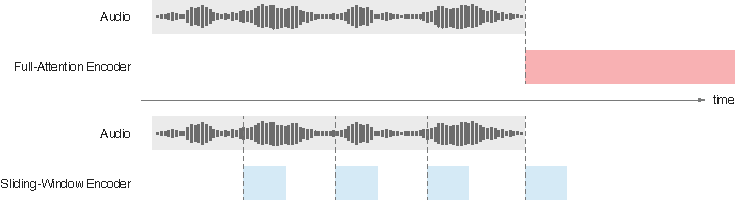
\includegraphics[width=\textwidth]{figures/encoder-comparison.pdf}
    \caption{Conceptual TTFT timelines. In full attention, encoding begins after the entire audio has arrived. With sliding-window attention, encoding proceeds incrementally and overlaps with audio capture, so the remaining work after the last chunk is smaller.}
    \label{fig:latency-timelines}
\end{figure*}
